\subsection{Защитный интервал в сетях LTE}
Рассмотрим систему, изображенную на рисунке~\ref{fig:vol_mobile_cell}.
\begin{figure}[H]
    \centering
    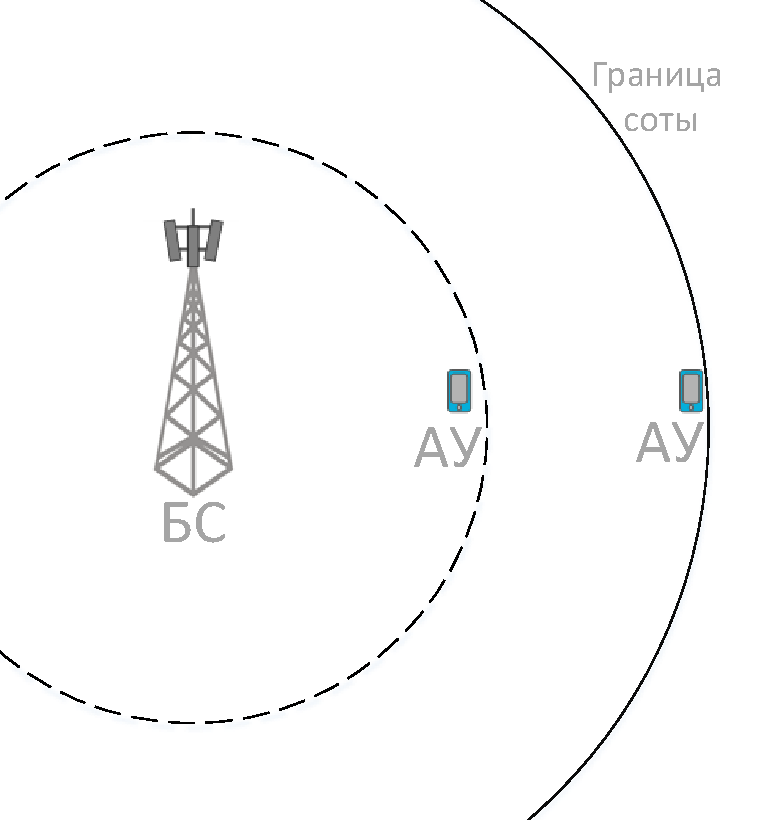
\includegraphics[width=0.5\textwidth]{img/vol_mobile_cell}
    \caption{Мобильная сота с двумя абонентами}
    \label{fig:vol_mobile_cell}
\end{figure}

Данная система состоит из базовой станции (БС) и двух абонентских устройств (АУ), один из которых
расположен непосредственно у базовой станции, второй --- на границе соты. Ни АУ, ни БС не могут знать
точное время появления данных в пределах установленного окна, так как информация передается с
некоторой задержкой. Если задержка одного из передаваемых сообщений окажется слишком большой, то
данное сообщение выйдет за границы собственного окна. Это может привести к наложению одного сообщения
на другое --- к интерференции, в результате которой принятые сообщения будет невозможно корректно
обработать. Подобный случай приведен на рисунке~\ref{fig:vol_interf}
\begin{figure}[H]
    \centering
    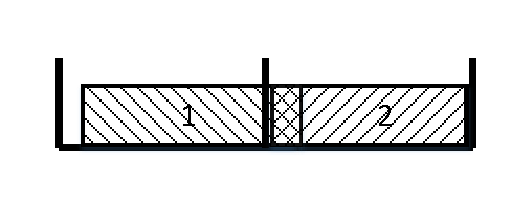
\includegraphics[width=0.5\textwidth]{img/vol_interf}
    \caption{Интерференция двух сообщений}
    \label{fig:vol_interf}
\end{figure}
Для устранения подобного эффекта вводится специальный параметр --- защитный интервал.
При использовании данного параметра время передачи сообщения сокращается. Освободившийся интервал
времени (защитный интервал) делится на две части: циклический префикс (ЦП) и защитное время (ЗВ).
ЦП является избыточной информацией и представляет собой повторение конца сообщения.
Он необходим для корректной обработки в тех случаях, когда сообщение вышло за границы
собственного окна. ЗВ необходим для того, чтобы снизить влияние задержки на передачу сообщений
абонентам, находящимся на больших расстояниях от базовой станции. Пример такого случая
приведен на рисунке~\ref{fig:vol_CP}. 
\begin{figure}[H]
    \centering
    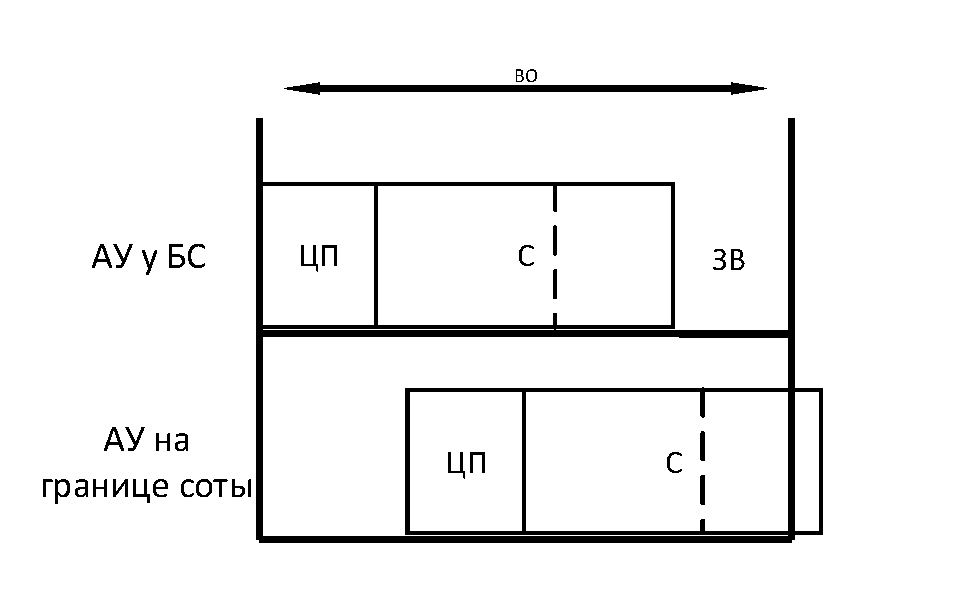
\includegraphics[width=0.75\textwidth]{img/vol_CP}
    \caption{Использование циклического префикса}
    \label{fig:vol_CP}
\end{figure}

Ошибки синхронизации, различные задержки при передаче сообщений приводят к интерференции.
Использование ЦП и ЗВ позволяет сократить возможность возникновения подобного явления.

Выбор размера ЦП и ЗВ во многом зависит от характера местности и размера соты. Для определения
влияния размера соты на значение ЦП рассмотрим рисунок~\ref{fig:vol_calc_CP}.
\begin{figure}[H]
    \centering
    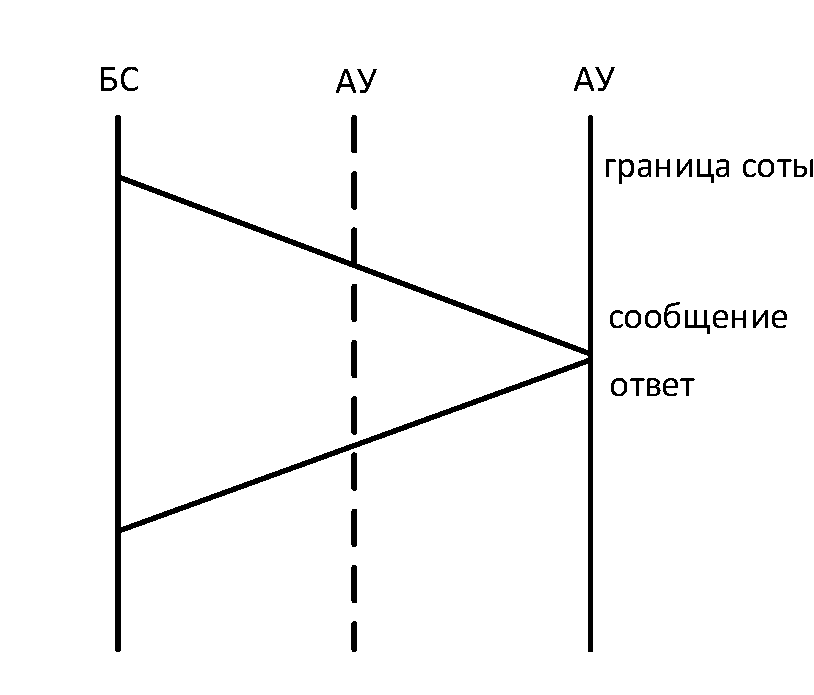
\includegraphics[width=0.5\textwidth]{img/vol_calc_CP}
    \caption{Передача сообщения от БС к АУ на границе соты}
    \label{fig:vol_calc_CP}
\end{figure}

Известно, что радиосигнал распространяется со скоростью примерно равной скорости света \(c = 3 \cdot
10^{8}\) м/с. Таким образом, время распространения сигнала от БС до дальнего АУ равно
\(T = \dfrac{Cell Size}{c}\). Но для завершения передачи БС должна получить ответ от АУ.
Время распространения ответа равно времени распространения сообщения \(T = \dfrac{2 \cdot Cell
Size}{c}\). Таким образом, через время, равное \(Т\), сообщение поступит на АУ, а спустя небольшую
задержку поступят переотраженные сигналы \((d)\).
Отсюда можно сделать вывод, что размер защитного интервала должен быть равен времени распространения
сигнала. В итоге размер циклического префикса равен \[T_{CP} = T = \dfrac{2 \cdot Cell Size}{c} + d\].

